\documentclass{article}
\usepackage{amsmath,amssymb,amstext,mathtools,array,url,bm,graphicx,color,epsfig}
\usepackage{fullpage,setspace}
\usepackage{authblk}
\usepackage{filecontents}
\usepackage{natbib}
\usepackage{lineno}
\usepackage[colorlinks]{hyperref}
\usepackage{subcaption}
\usepackage{float}
\usepackage[flushleft]{threeparttable}

\def\dt{\partial t}
\def\dx{\partial x}
\def\dy{\partial y}

\def\dz{\partial z}
\def\BE{\begin{equation}}
\def\EE{\end{equation}}
\def\half{\frac{1}{2}}
\def\calT{\cal T}
\def\Deltax{\Delta x}
\def\Deltat{\Delta t}
\DeclareSymbolFont{largesymbolsA}{U}{txexa}{m}{n}
\DeclareMathSymbol{\varprod}{\mathop}{largesymbolsA}{16}

\newtheorem{theorem}{Theorem}
\newtheorem{acknowledgement}[theorem]{Acknowledgement}
\newtheorem{algorithm}[theorem]{Algorithm}
\newtheorem{axiom}[theorem]{Axiom}
\newtheorem{case}[theorem]{Case}
\newtheorem{claim}[theorem]{Claim}
\newtheorem{conclusion}[theorem]{Conclusion}
\newtheorem{condition}[theorem]{Condition}
\newtheorem{conjecture}[theorem]{Conjecture}
\newtheorem{corollary}[theorem]{Corollary}
\newtheorem{criterion}[theorem]{Criterion}
\newtheorem{definition}[theorem]{Definition}
\newtheorem{example}[theorem]{Example}
\newtheorem{exercise}[theorem]{Exercise}
\newtheorem{lemma}[theorem]{Lemma}
\newtheorem{notation}[theorem]{Notation}
\newtheorem{problem}[theorem]{Problem}
\newtheorem{proposition}[theorem]{Proposition}
\newtheorem{remark}[theorem]{Remark}
\newtheorem{solution}[theorem]{Solution}
\newtheorem{summary}[theorem]{Summary}
\newenvironment{proof}[1][Proof]{\noindent\textbf{#1.} }{\ $\square$}


\begin{document}
\section*{Deleted paragraphs related to wrong local speed estimates}

\section{Small scale flows on inclined plane and flat runway}
\subsection{Flow speed}
Figure \ref{fig:Ramp-Vel} shows the flow speed, $\Vert \underline{\mathbf{u}} \Vert(L,t)$, at the points $(L_i)_{i=1,\dots,4}$, for the three rheology models.
\begin{figure}[H]
         \centering
        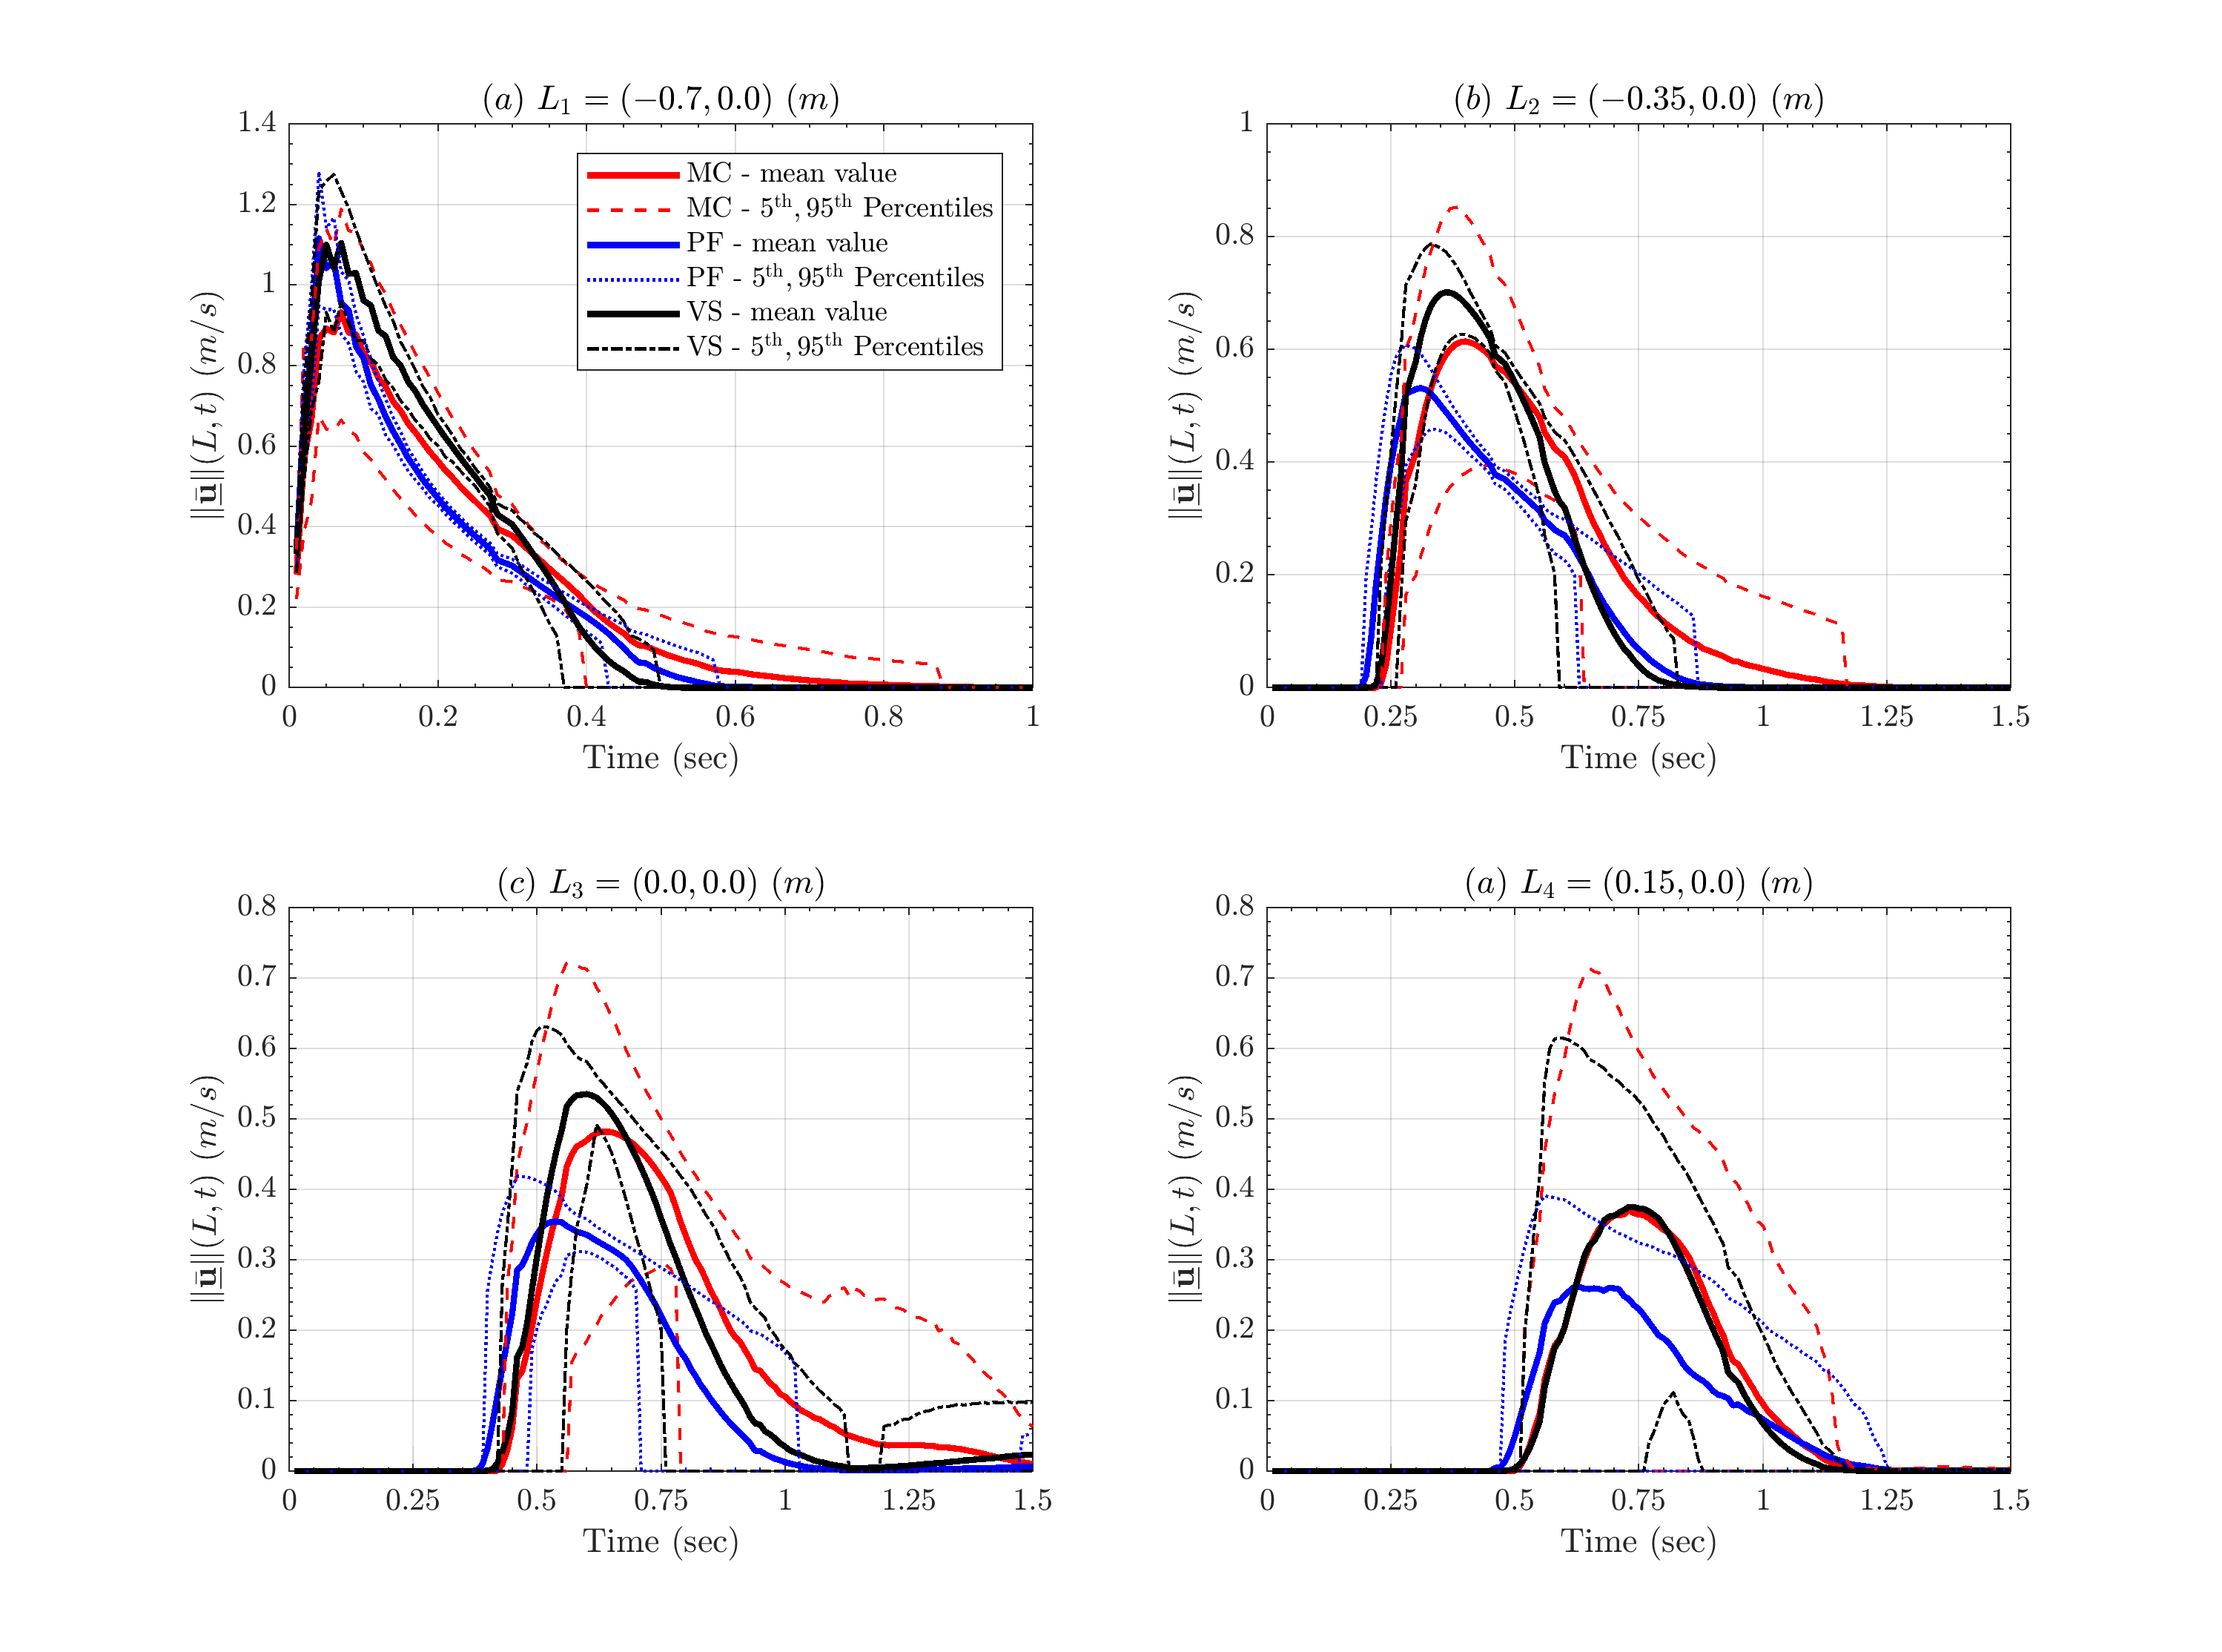
\includegraphics[width=1\textwidth]{InclinedPlane/LocalMeasurments/Velocity_Inc.png}
        \caption{Records of flow speed at four spatial locations of interest. Bold line is mean value, dashed/dotted lines are 5$^{\mathrm{th}}$ and 95$^{\mathrm{th}}$ percentile bounds. Different rheology models are displayed with different colors. Plots are at different scale.}
        \label{fig:Ramp-Vel}
\end{figure}
In plot \ref{fig:Ramp-Vel}a related to point $L_1$ speed peaks are $0.95 \pm 0.3$ m/s in MC, $1.1 \pm 0.2$ m/s in VS and PF. VS speed decreases almost linearly, while MC and PF have a more concave profile, making MC the faster model after $0.3$ sec. Plot \ref{fig:Ramp-Vel}b, related to point $L_2$, the peaks are $0.65 \pm 0.2$ m/s in MC, $0.7 \pm 0.1$ m/s in VS, and $0.52 \pm 0.08$ m/s in PF. In this case it is the PF model to decrease more linearly. In plot \ref{fig:Ramp-Vel}c, related to point $L_3$, peak velocity is $0.48$, $[+0.24, -0.20]$ m/s in MC, $0.54$, $[+0.1, -0.06]$ m/s in VS, and $0.36$, $[+0.06, -0.04]$ m/s in PF. In plot \ref{fig:Ramp-Vel}d, related to point $L_4$, peak velocity is $0.48$, $[+0.34, -0.48]$ m/s in MC, $0.48\pm 0.24$ m/s in VS, and $0.26$, $[+0.12, -0.26]$ m/s in PF. In all cases UQ shows that MC model uncertainty is remarkably larger than in the other models, and produces higher values in the 95$^{\mathrm{th}}$ percentile plots. Lowest speed values are affected by the elimination of material below $1$ mm flow height threshold. After $0.05$ s, the PF velocity profile is always significantly lower than the other models, but it also decreases slower, and matches with the stopping times of them. Moreover, it is worth noting that, curiously, PF reaches the points earlier. Speed in the deposits is below $0.1$ m/s in $L_3$, negligible in $L_4$.

\section{Large scale flows on the SW slope of Volc{\'a}n de Colima (MX)}
\subsection{Flow speed - overview}
Figure \ref{fig:BAF-V-MC} shows the mean flow speed, $h(L,t)$, at the 51 spatial locations of interest, according to MC.
\begin{figure}[H]
         \centering
        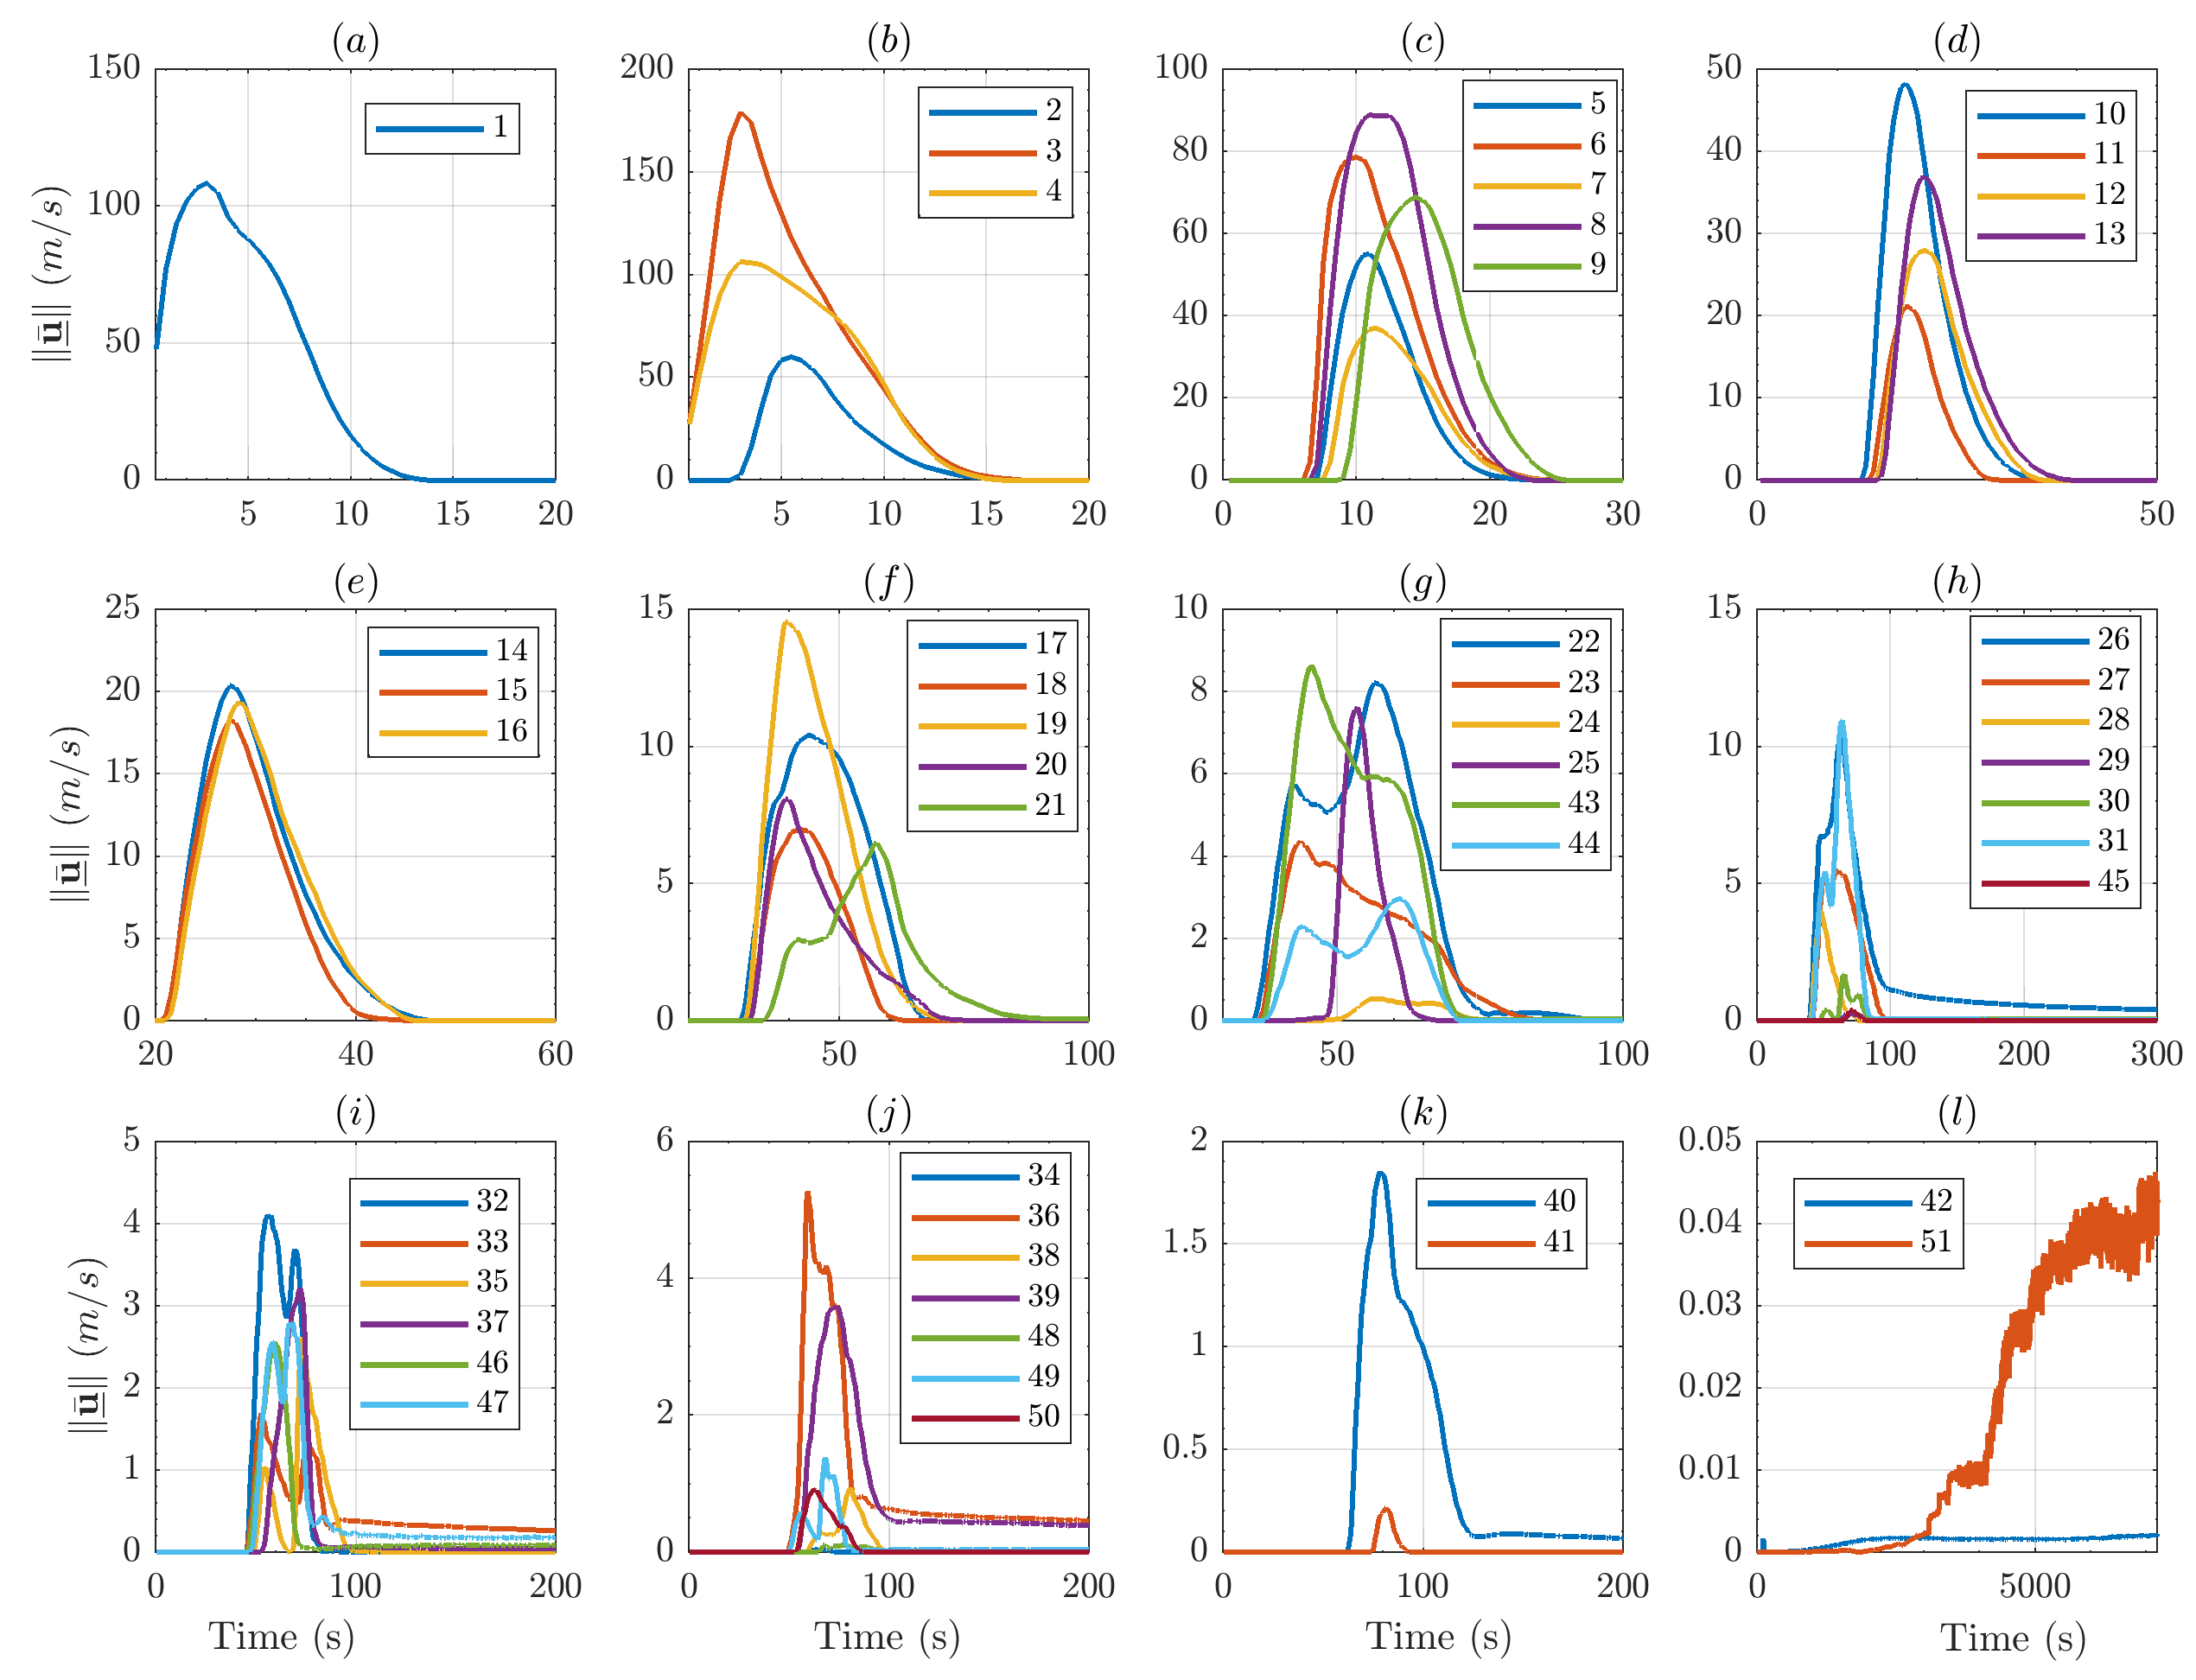
\includegraphics[width=1\textwidth]{MC&VS_51/Velocity_MC3.png}
        \caption{MC model, records of average flow speed, $\vert\underline{u}\vert(L,t)$, in 51 spatial locations of interest.}
        \label{fig:BAF-V-MC}
\end{figure}
Again the different plots have different scales on either time and space axes. The plot profiles are similar to what observed in figure \ref{fig:Ramp-Vel}, following the plot profile classification described above. Maximum speed of $\sim 200 m/s$ is observed in proximity of the initial pile, in plot \ref{fig:BAF-V-MC}b, and it is related to the initiation collapse dynamics. After 1 km runout (horizontal projection), in plot \ref{fig:BAF-V-MC}e, the max speed is ten times smaller, $\sim 20 m/s$. At about 2 km from the initiation, when entering the main ravines, speed is $\sim 10 m/s$, and becomes $\sim 5 m/s$ or less in the distal part of the ravines.  In detail, in plots  \ref{fig:BAF-V-MC}f,g,h,i,j, the speed often shows bimodal profiles, not observed in the inclined plane case study. Moreover, in plots \ref{fig:BAF-V-MC}h,i,j, positive asymptotes are sometimes observed, meaning a slowly and steadily moving material even minutes after the collapse.

\subsection{Flow speed - six selected points}
Figure \ref{fig:Colima-Vel} shows the flow speed, $\Vert \underline{\mathbf{u}} \Vert(L,t)$, at the points $(L_i)_{i=8,10,17,39,43,46}$, for the three rheology models. Pairs of points $L_8$ and $L_{10}$, points $L_{17}$ and $L_{43}$, and points $L_{39}$ and $L_{46}$ have significantly similar plot profiles. In plot \ref{fig:Colima-Vel}a MC shows higher average speed, $\sim 80 m/s$, than PF and VS, both $\sim 70 m/s$. 95$^{th}$ percentile values can reach $150 m/s$ in MC, $140 m/s$ in VS, $130 m/s$ in PF. MC and PF are null after $20 s$, while VS decreases slower, and becomes null at $\sim 60 s$. In plot \ref{fig:Colima-Vel}b, the average peak values are $\sim 40 m/s$ in MC and PF, while only $20 m/s$ in VS. All the three models show 95$^{th}$ percentile values above $60 m/s$. VS speed decreases remarkably slower than in the other models, requiring more than $120 s$ to become null, while MC and PF speed remains positive for $\sim 25 s$. In plot \ref{fig:Colima-Vel}c, average speed is $\sim 20 m/s$ in PF, $\sim 10 m/s$ in MC, $\sim 2 m/s$ in VS. 95$^{th}$ percentile values can reach $\sim 55 m/s$ in PF, $\sim 48 m/s$ in MC, $\sim 24 m/s$ in VS. The duration of positive velocity in VS can be long hundredths of seconds. 
\begin{figure}[H]
         \centering
        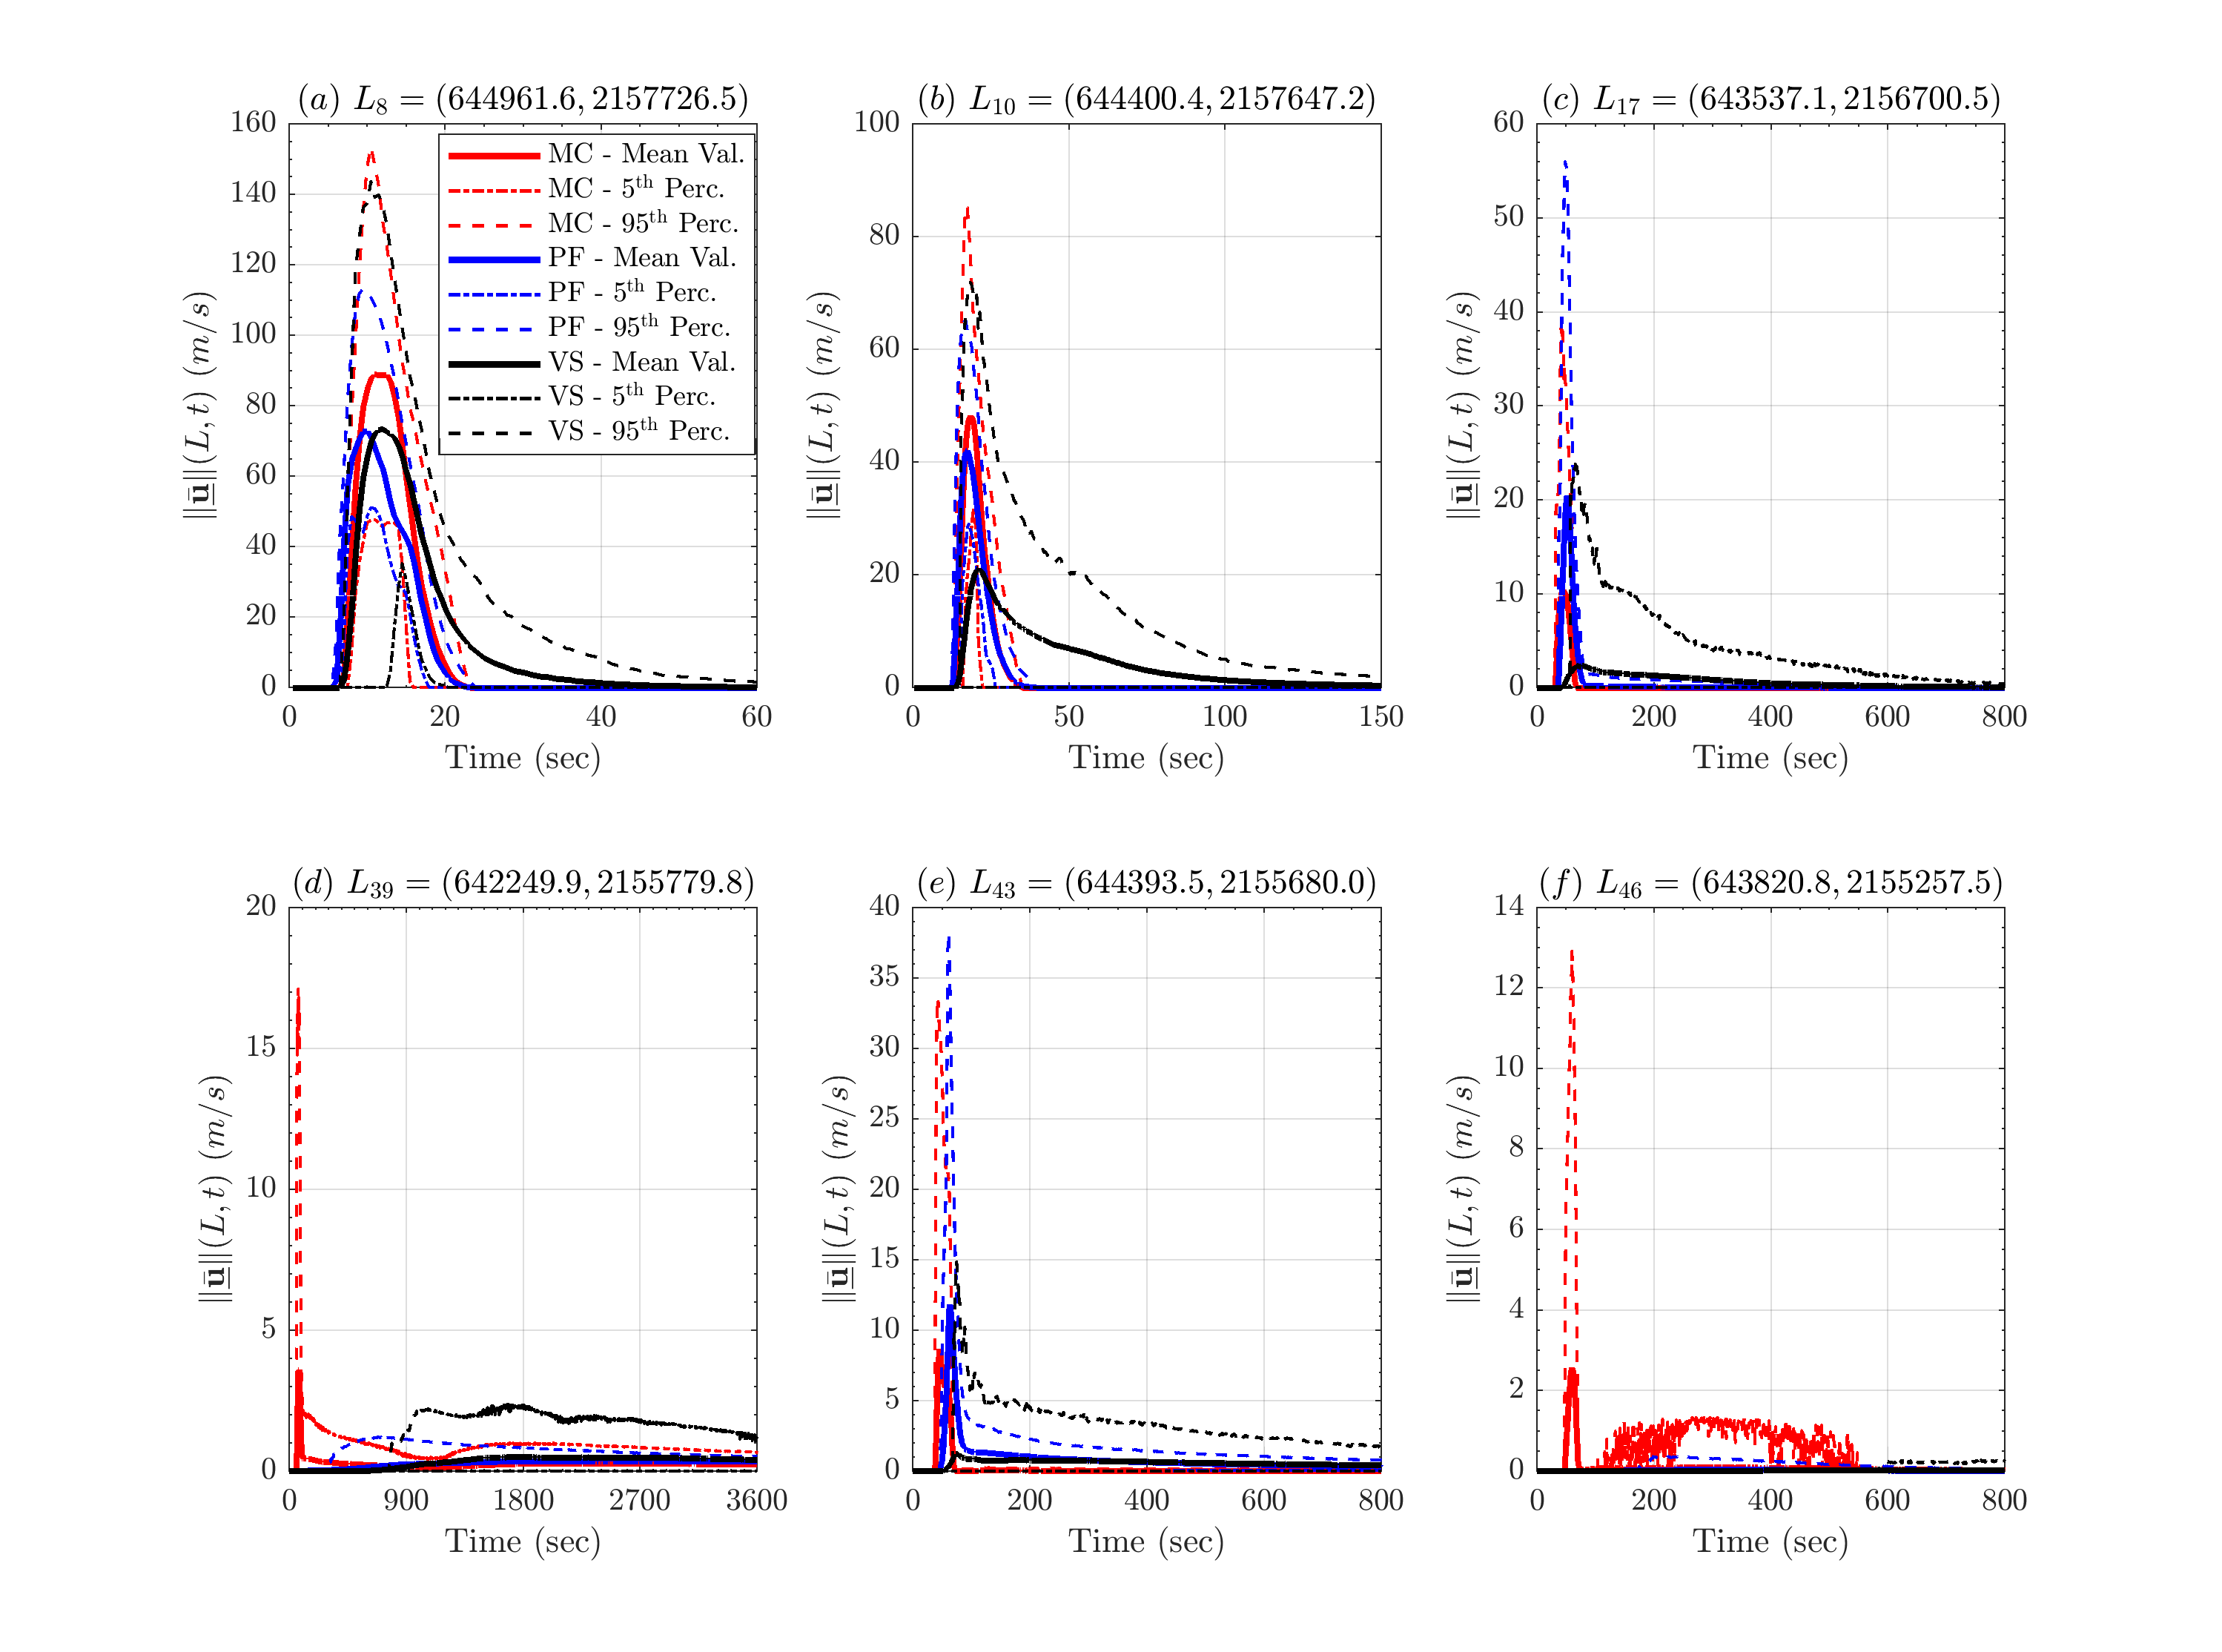
\includegraphics[width=1\textwidth]{BAF_VolcanDeColima/LocalMeasurments/Velocity_Col.png}
        \caption{Records of flow speed at six selected locations. Bold line is mean value, dashed/dotted lines are 5$^{\mathrm{th}}$ and 95$^{\mathrm{th}}$ percentile bounds. Different rheology models are displayed with different colors. Plots are at different scale. Numerical noise affecting percentile curves in (f) has been averaged.}
        \label{fig:Colima-Vel}
\end{figure}
A very similar situation is pictured in plot \ref{fig:Colima-Vel}e. Instead in plot \ref{fig:Colima-Vel}d, only MC shows a max speed above $3 m/s$, the 95$^{th}$ percentile values at $\sim 15 m/s$. In the other models the average speed is always below $1 m/s$ and the 95$^{th}$ percentile values have an increasing profile followed by a slightly decreasing plateau, at $\sim 2 m/s$ in VS, $\sim 1 m/s$ in PF. VS can have a speed above $\sim 1 m/s$ at $\sim 3600 s$. In plot \ref{fig:Colima-Vel}f, only MC shows an average speed above zero, while in the other models even the 95$^{th}$ percentile values are always below $\sim 0.5 m/s$, and start to be positive only at $\sim 200 s$ in PF, and $\sim 600 s$ in VS. MC can have speed at $\sim 1 m/s$ for more than $\sim 500 s$, but the plot is very noisy.

\section{Discussion}
\subsection{Flow speed}
Flow speed enriches our analysis of additional details. In Fig. \ref{fig:Ramp-Vel} MC has a fatter tail, due to the already observed distal spreading of material. PF profile is more concave at the beginning, due to the combined effects of the dual bed friction angle and the hydrostatic correction. In Fig. \ref{fig:Colima-Vel} VS is confirmed to be significantly slower than the other models, after the initial collapse. Moreover, it is the only model which presents slowly moving material for all the simulation, near the initiation pile. MC shows short lasting peaks of speed even in the most distal sample points, due to the lack of a strong slowing mechanism like the secondary angle in PF, and the speed dependent term in VS.
\end{document}




















